\section{Muon-in-jet + pt reco}

\subsection{Jets}
\label{subsec:jets-analysis}

Jets are clustered using the anti-\kt algorithm with a distance parameter of R = 0.4 \cite{Cacciari:2008gp}.
This analysis uses jets clustered from particle-flow (PFlow) objects which improves the jet resolution at low \pT by capitalizing on the excellent resolution of the tracker to better estimate the energy of low \pT clusters \cite{PERF-2015-09}.  
The jet energy and direction is corrected to account for contamination from the underlying pile-up distribution, fluctuations due to the origin of the jet and its stochastic fluctuations, and residual differences between data and MC \cite{JETM-2018-05}.
The file used for applying this Jet Energy Scale (JES) calibration is: \\
{ \tt JES\_MC16Recommendation\_Consolidated\_PFlow\_Apr2019\_Rel21.config}.

To suppress the contribution of jets formed by pile-up processes, jets with \pT~<~60~\GeV~and $|\eta|$~<~2.4 are required to pass a Jet Vertex Tagger (JVT) cut \cite{ATLAS-CONF-2014-018}. The (default) tight working point is considered, as it is 96\% efficient for hard scatter jets \cite{jvt-twiki}.
Jets produced by cosmic-rays, beam-induced background, and out-of-time pileup are reduced by imposing a set of quality criteria on variables characterizing the jet profile \cite{ATLAS-CONF-2015-029}. Jets considered for these cleaning cuts are clustered from calorimeter clusters (EMTopo jets) and have \pT~>~20~GeV, since these variables defining the jet cleaning cuts depend on the jet collection, and the recommendation was optimized for EMTopo jets \cite{jet-cleaning-twiki}. 
If a single jet in the event fails the (default) {\tt LooseBad} jet quality criterion, the entire event in vetoed. This recommendation is implemented via the {\tt DFCommonJets\_eventClean\_LooseBad} variable in the EXOT8 derivation.

This analysis makes use of PFlow jets with $|\eta| < 4.5$ and \pT down to 30~\GeV. 
Since the Jet/ETMiss group does provide calibrations down to 20~\GeV, jets with a lower \pT cutoff were studied, but not found to improve the analysis's sensitivity due the exponential increase of multi-jet background. 

\subsection{\Pqb-tagging}
\label{subsec:ftag-analysis}


\Pqb-jets are identified by the neural network-based DL1r algorithm with inputs characterizing the displaced tracks and vertices of the weakly decaying \Pqb-hadron \cite{FTAG-2018-01}. 
This newly recommended DL1r algorithm improves on the previously recommended BDT-based algorithm, MV2c10, by including a Recurrent Neural Network to account for the correlation between the tracks in the jet \cite{ATL-PHYS-PUB-2017-003}.

For the \Pqb-tagging working-point optimization, both the MV2c10 and DL1r algorithms used dedicated trainings on the newly recommended PFlow jet collection \cite{PFlowPublicPlots2019}.
The higher background rejection of DL1r allowed for a loosening of the b-tagging working point from 70\% to 77\% with a corresponding 10\% improvement in the stat-only ggF SM limits. 
The decision to move to the 77\% working point was made in harmony with the other HH channels for ease in the subsequent combination.

In the context of the future combination, since the majority of the HH analyses include $b$-jets in the final state, other channels are vetoing events with three DL1r \Pqb-tags at the 77\% WP jet in the combination (to conservatively also veto our 4b events, and give us the possibility to explore a 3b analysis category).

\subsection{\Pqb-jet corrections}
\label{subsec:regression}

The jet calibrations described in \Sect{\ref{subsec:jets-analysis}} focus on corrections for light-quark and gluon-initiated jets.
As such, they systematically underestimate the energy of \Pqb-jet due to two main effects.
\begin{enumerate}
	\item When the \Pqb-hadron decays semi-leptonically with a $W \rightarrow \mu \nu_\mu$ interaction in the cascade, % (which happens 11\% of the time)
	\begin{itemize}
		\item the neutrino energy is invisible in the jet reconstruction, and
		\item the muonic energy is only partially accounted for in the jet's energy estimate since the muon ($\mu$) is not stopped in the calorimeter.
	\end{itemize}
	\item The \Pqb-jet fragmentation is wider than that of the corresponding light-jets, meaning fewer final state hadrons from the \Pqb-quark fragmentation are included in jet clustering reconstruction (``out-of-cone'' effect).  
		
\end{enumerate}

To correct for these effects, the HH analyses employ a harmonized $\mu$-in-jet~+~\pT-reco correction to account for this underestimation of the \Pqb-jet \pT. 
This centralized \Pqb-jet correction is more sophisticated than the previous ggF correction of simply adding back in $\mu$ 4-vectors within $\Delta R < 0.4$ of the jet axis, although the previous VBF analysis did have a dedicated BDT-based \Pqb-jet energy regression \cite{HDBS-2018-18-witherratum}.  
The $\mu$-in-jet~+~\pT-reco algorithm is implemented centrally by the \texttt{BJetCalibrationTool} \cite{BJetCalibrationTool}, and a brief description is given below.

\subsubsection{$\mu$-in-jet}

A search for a $\mu$ is performed in a variable radius cone $\Delta R(\mu, \text{jet}) < \min \left( 0.4, 0.04 + 10 / p_T^{\mu} \ \text{GeV} \right)$\footnote{The $\min$ function selects which of its arguments is smallest, and its use here avoids adding a $\mu$ farther away from the jet axis than the jet clustering distance parameter.} from the jet axis to account for the increasingly collimated decay products of more energetic jets.
If a $\mu$ is identified at the medium working point with \pT~>~4~GeV, $|\eta|$~<~2.5 is within this $\Delta R$ cone of the jet axis, its 4-vector is added to that of the jet. If there are multiple $\mu$s passing the above criteria, only the $\mu$ closest to the jet-axis is added. Then the expected energy that the $\mu$ lost in the calorimeter is subtracted since this contribution was already included in the jet energy estimate.

\subsubsection{\pT-reco}

This second step accounts for the missing neutrino energy and out-of-cone effects that Jet/ETMiss calibrations don't capture.
This correction factor is derived in $t\bar{t}$ events to correct the reconstructed \pT of the \Pqb-jets in logarithmic bins of the truth jet \pT. 
Since the correction is larger for \Pqb-jets decaying semi-leptonically, these correction factors are derived separately for \Pqb-jets with and without a $\mu$. 

\Fig{\ref{fig:bjetcalib-plots}} illustrates the improvement achieved by the \Pqb-jet corrections in $m_{\PH1}$, $m_{\PH2}$ and \mhh resolusion.

\def\figpath{figures/nr-int-note/objects/V1/}

\begin{figure}[hb]
	\centering
	\subfloat[$m_{\PH1}$]{ 
	    	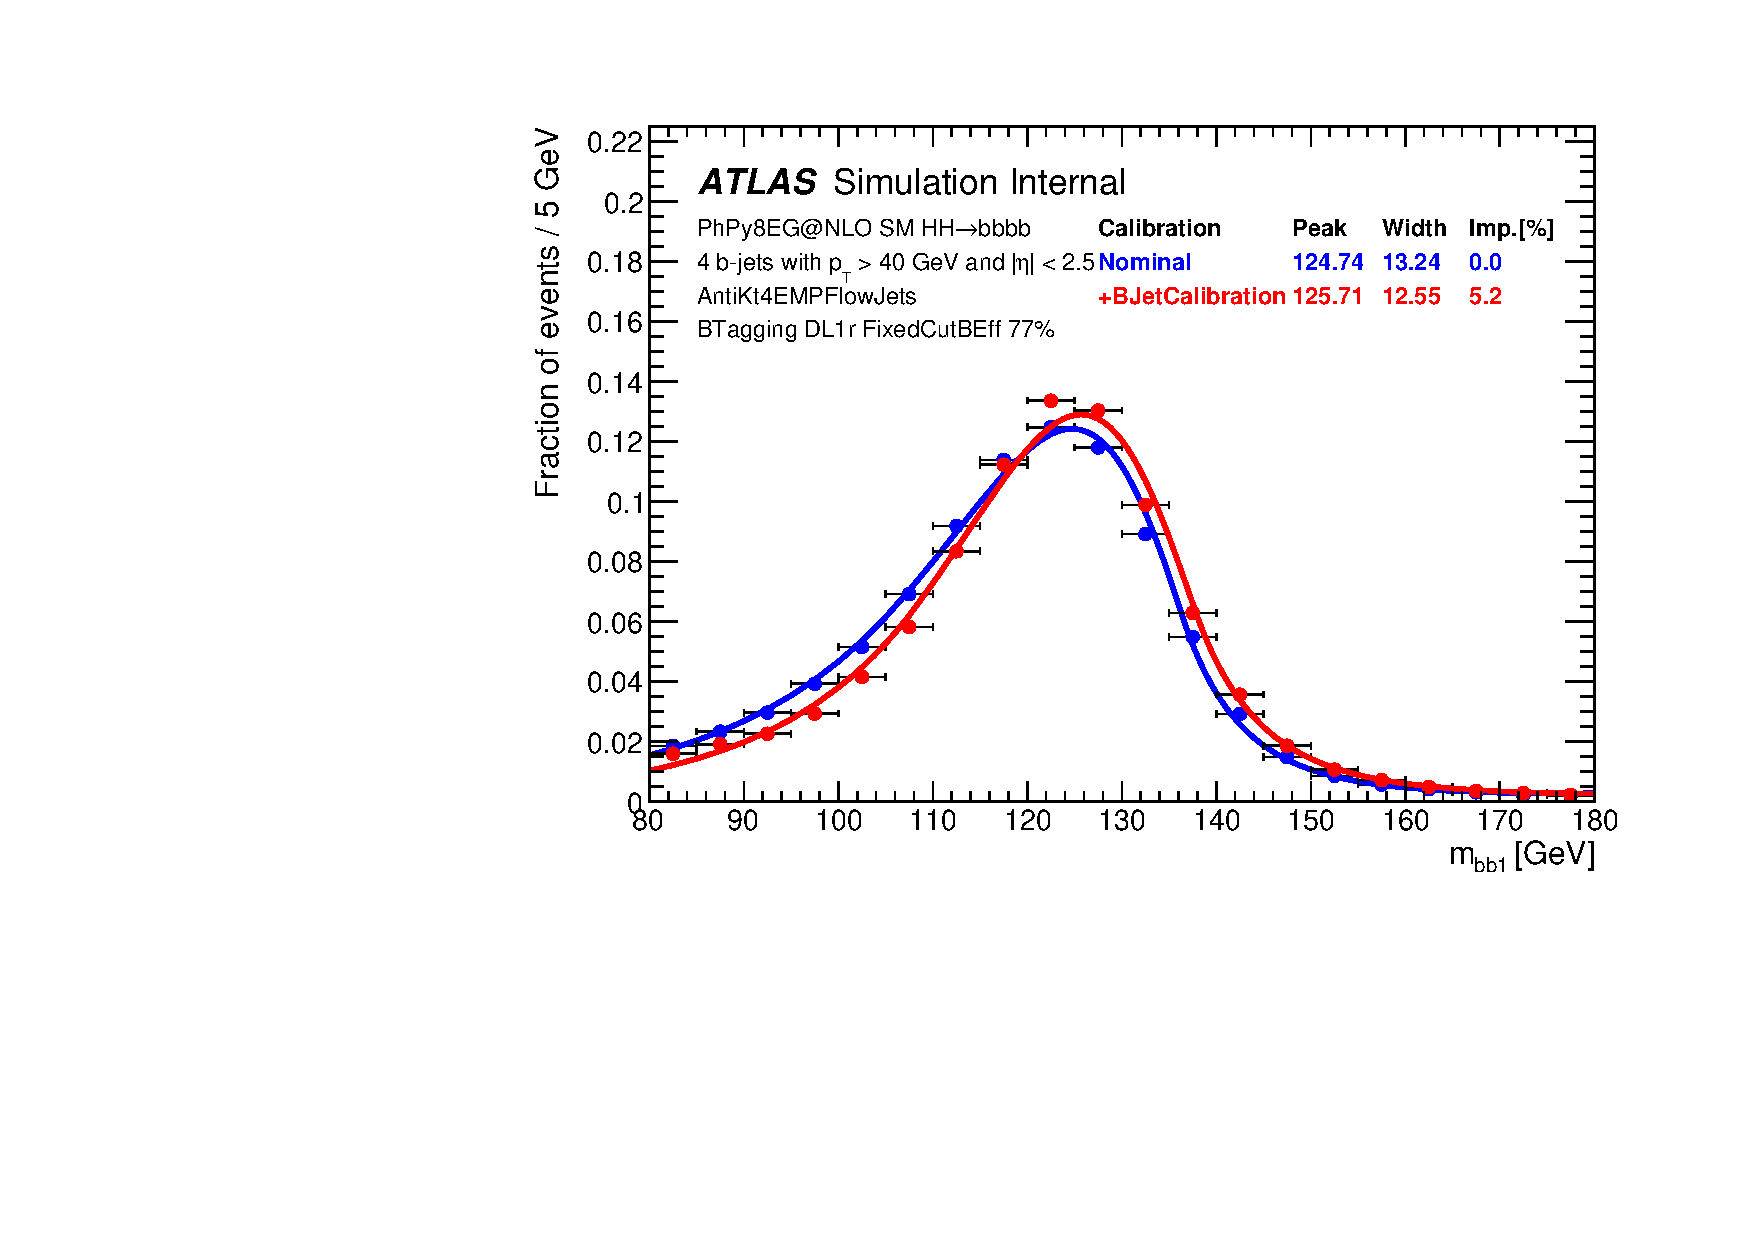
\includegraphics[width=0.33\textwidth]{\figpath/MAY21-Qs45-bjetcalib-Everything-18-m-h1-4b.pdf}
		\label{fig:bjetcalib-mh1}
	} 
	\subfloat[$m_{\PH2}$]{ 
	    	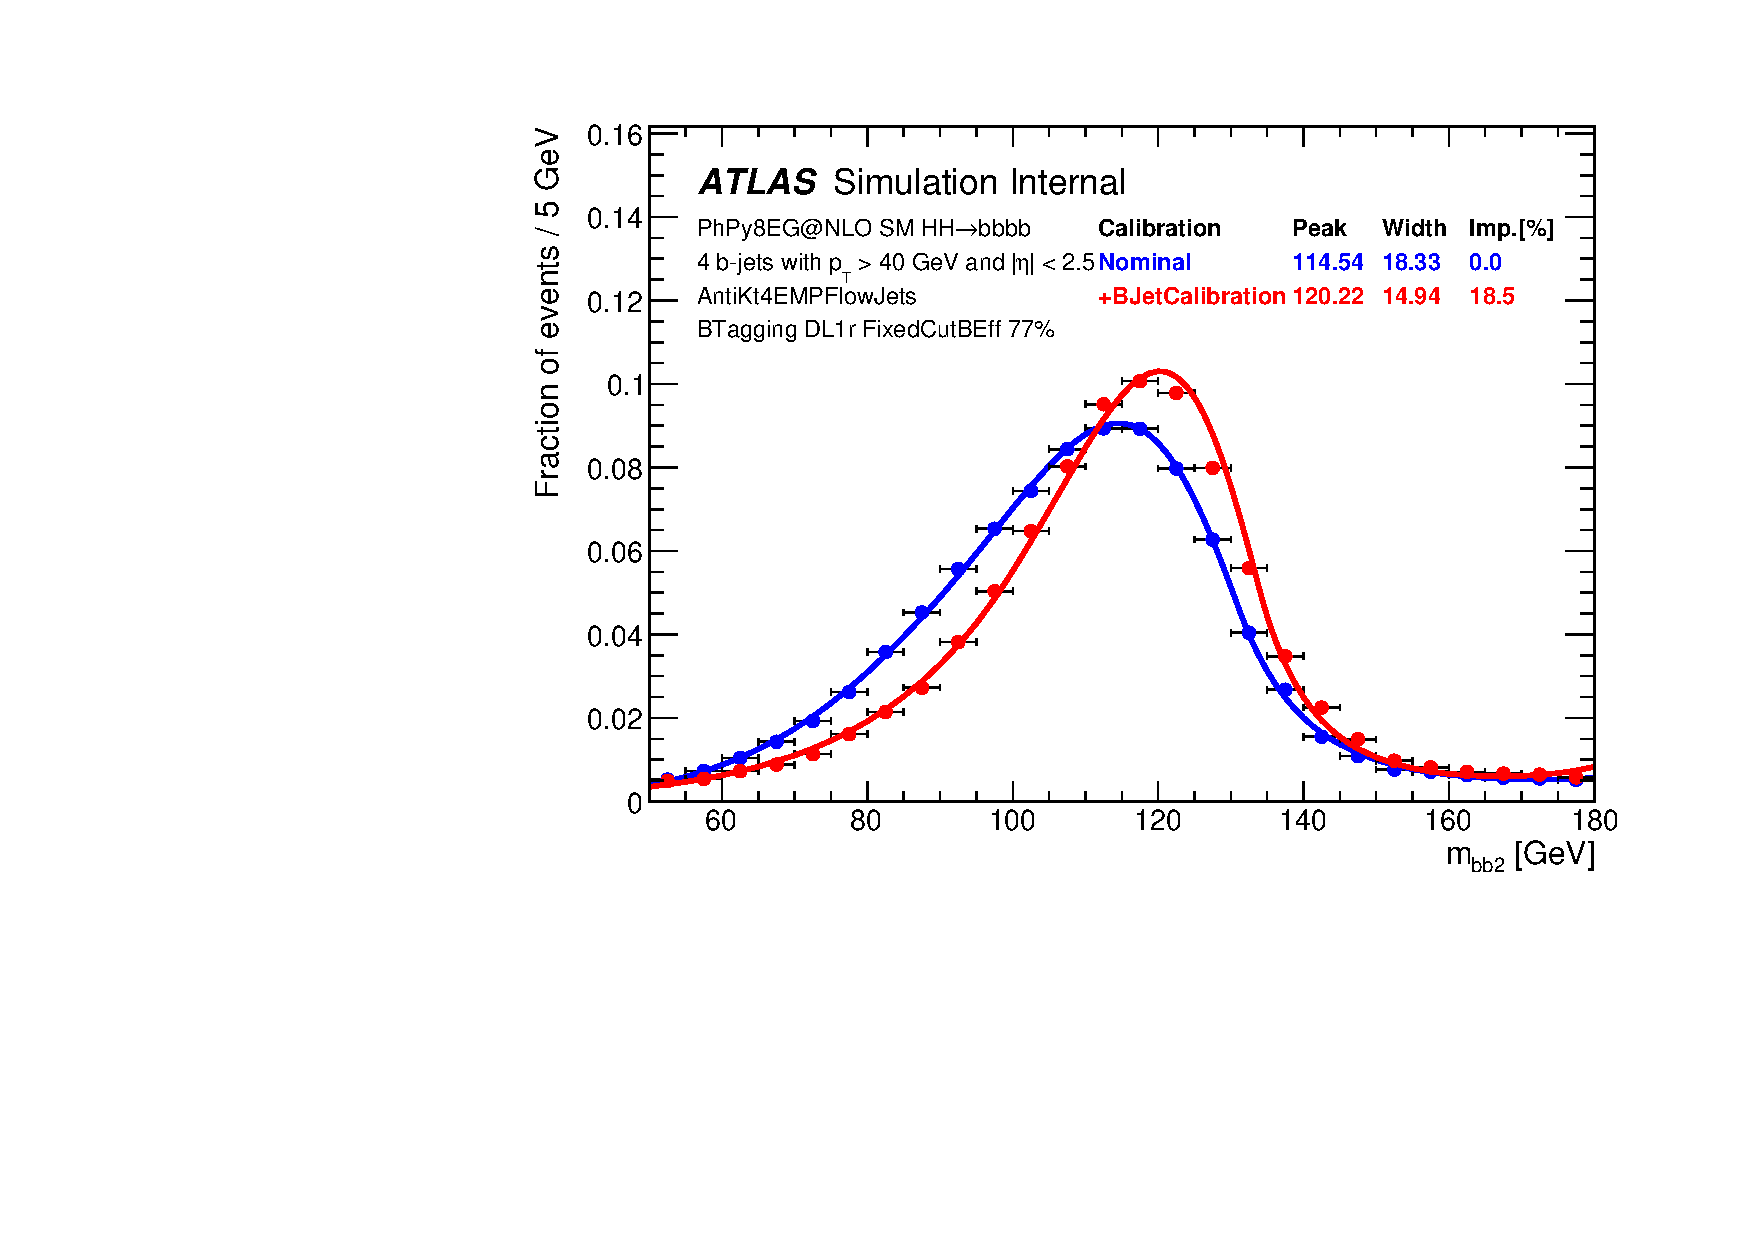
\includegraphics[width=0.33\textwidth]{\figpath/MAY21-Qs45-bjetcalib-Everything-18-m-h2-4b.pdf}
		\label{fig:bjetcalib-mh2}
	} 
	\subfloat[\mhh]{ 
	    	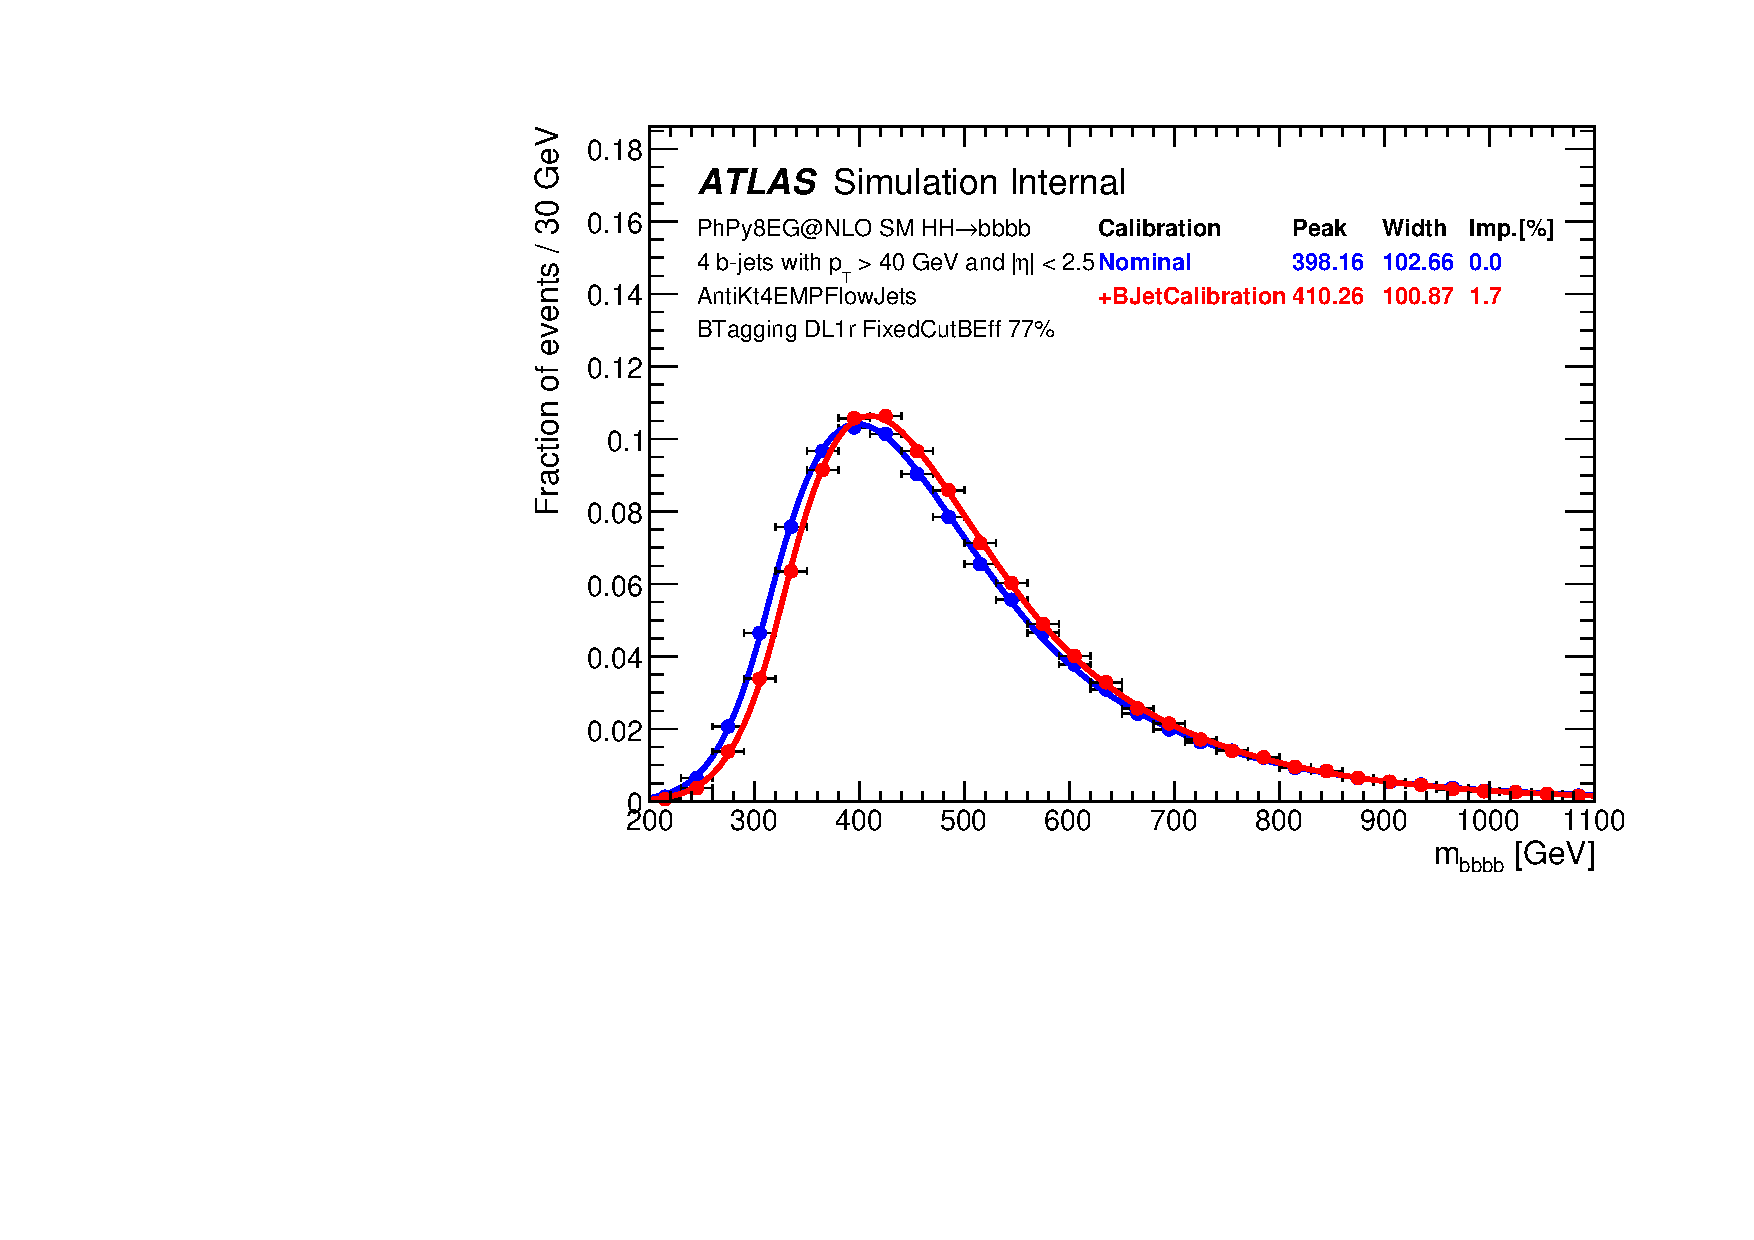
\includegraphics[width=0.33\textwidth]{\figpath/MAY21-Qs45-bjetcalib-Everything-18-m-hh-4b.pdf}
		\label{fig:bjetcalib-mhh}
	} 

	\caption{Comparisons of $m_{\PH1}$, $m_{\PH2}$ and \mhh distributions before the \Pqb-jet corrections~(blue) and 
                 after the \Pqb-jet corrections~(red). These distributions are fitted using Bukin function, and the peak, 
                 the peak resolusion and the relative improvement are shown in the legend.}
	\label{fig:bjetcalib-plots}
\end{figure}


